\section{Results}

\begin{figure}[ht]
  \centering
  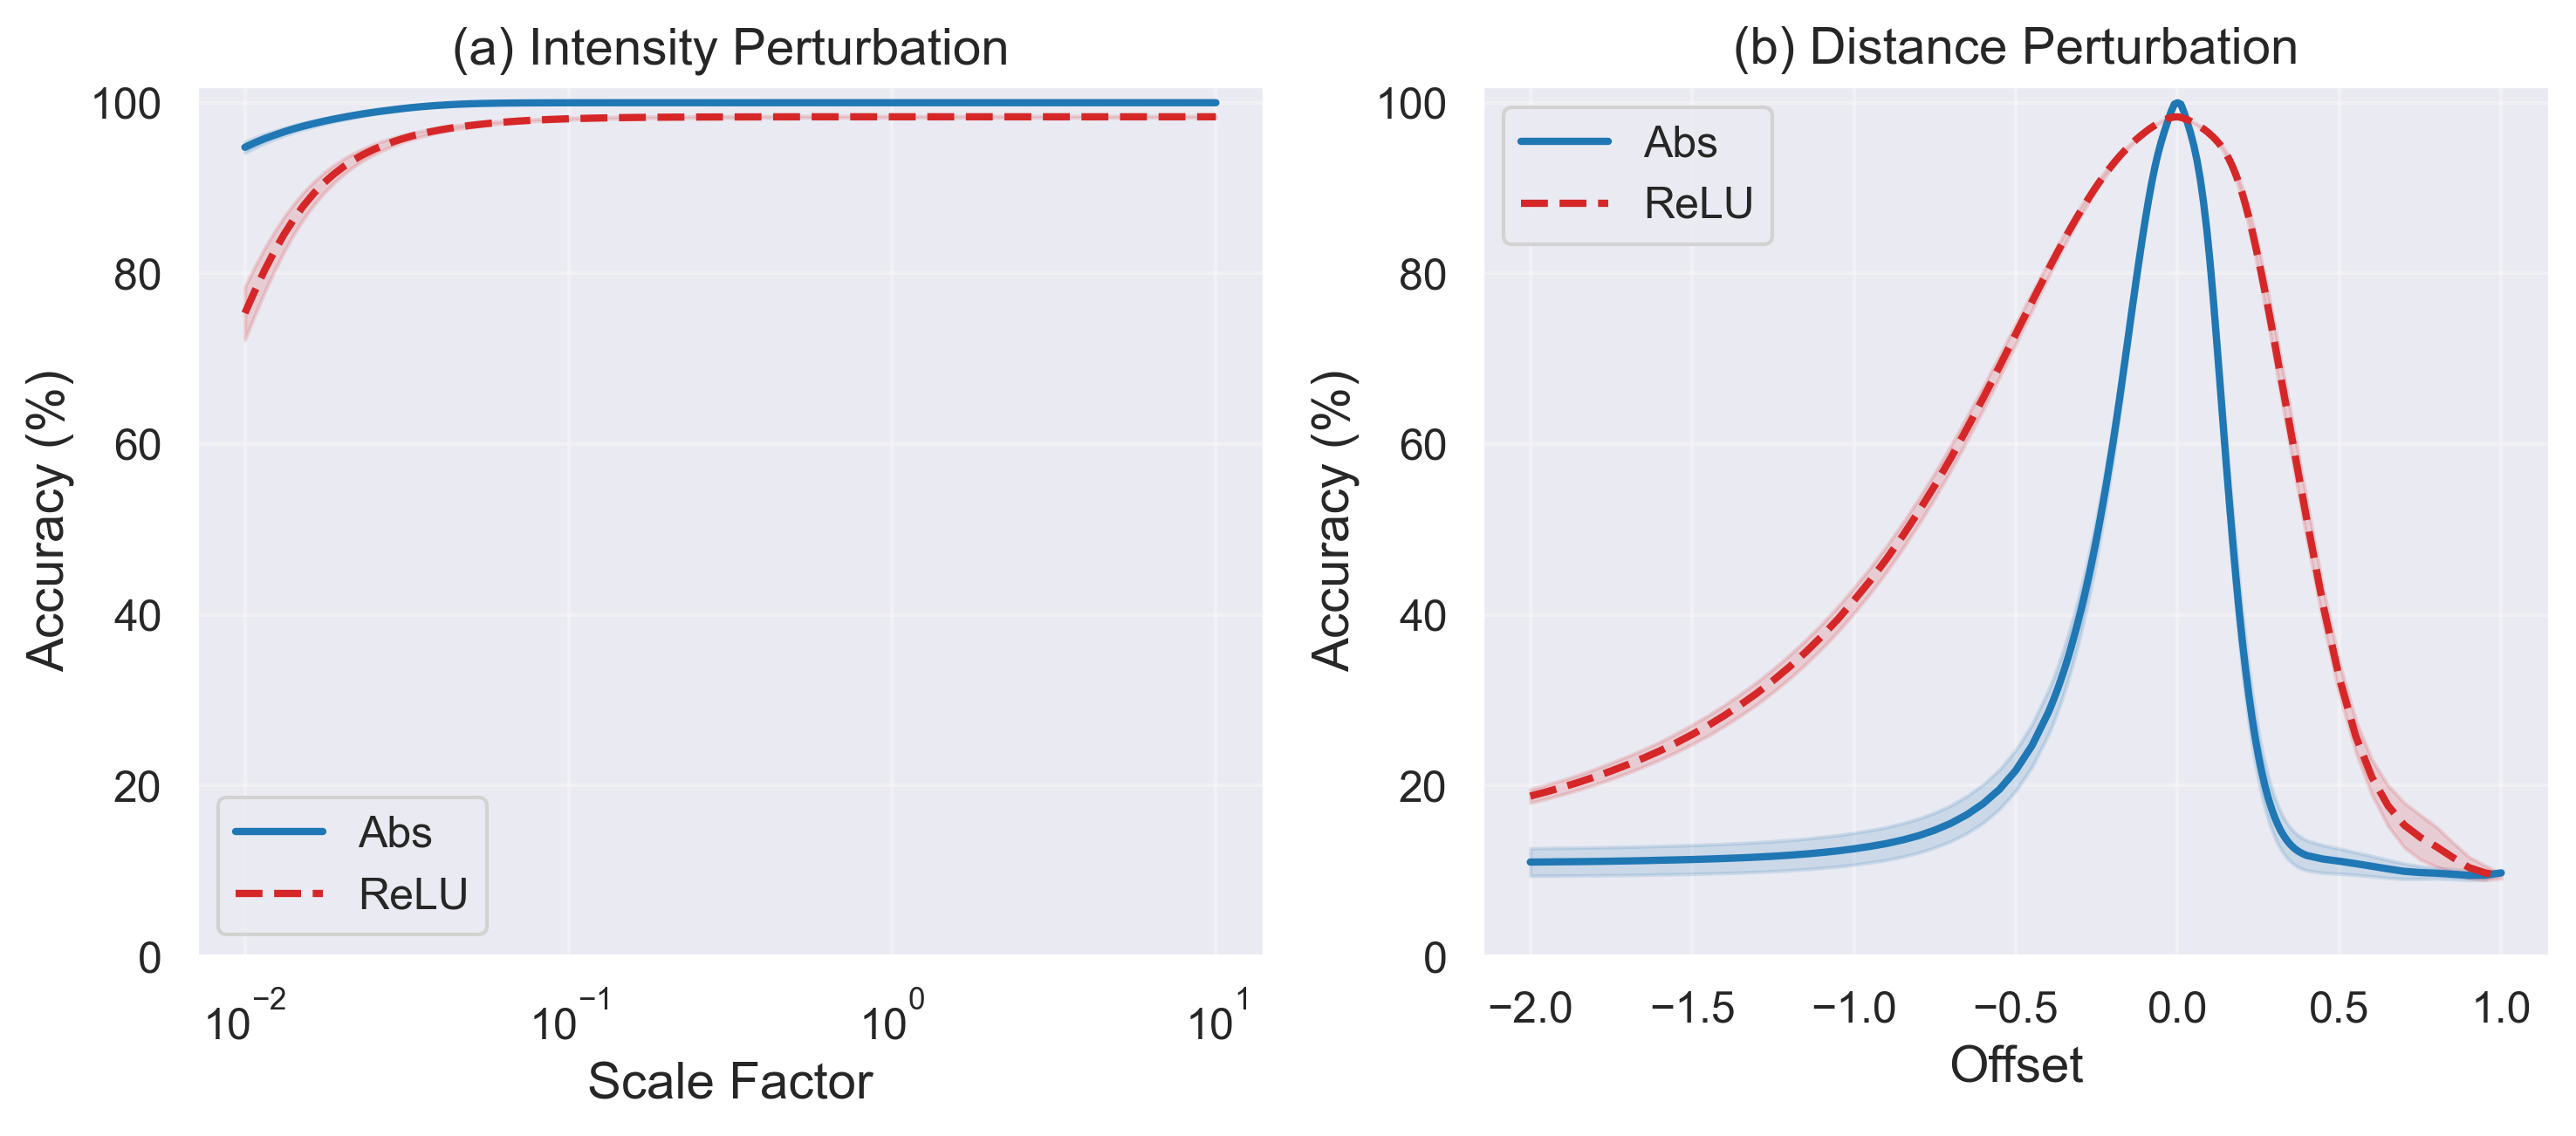
\includegraphics[width=\textwidth]{images/perturbation_analysis}
  \caption{Effects of intensity scaling and distance offset perturbations on model accuracy. Shaded regions represent 95\% confidence intervals across 20 runs.}
  \label{fig:perturbation_analysis}
\end{figure}

Our experiments provide strong empirical support for the theory that the tested models (Abs and ReLU) primarily utilize \textit{distance metrics}, rather than \textit{intensity metrics}, for classification. This means that the models rely on features residing near the decision boundaries for classification, rather than in regions with high activation magnitudes. As shown in Table~\ref{tab:stat_baseline}, both models achieved high accuracy on MNIST \citep{lecun1998gradient} before perturbation testing. 

Consistent with our theory, both models demonstrate strong invariance to intensity perturbations while exhibiting significant sensitivity to distance perturbations (Figure~\ref{fig:perturbation_analysis}). Specifically, both models maintain their baseline accuracy (approximately 98\% for ReLU and 99\% for Abs) across a wide range of intensity scaling (from 10\% to 200\% of the original output range) and threshold clipping (from 50\% of the maximum activation and above). The minor fluctuations in accuracy observed within these ranges were small and not statistically significant (p > 0.05), as detailed in Table~\ref{tab:stat_scale} and Table~\ref{tab:stat_cutoff}. This robustness to intensity perturbations suggests that the models are not heavily reliant on the absolute magnitude of activations, or \emph{intensity metrics}, for classification. This aligns with findings in adversarial example literature, where imperceptible perturbations can drastically alter model predictions \citep{szegedy2013intriguing, goodfellow2014explaining}.

In contrast, both models exhibit a rapid decline in accuracy with relatively small distance offset perturbations. ReLU maintains its baseline accuracy over an offset range from -3\% to +2\% of the activation range, while the Abs model is even more sensitive, falling below 99\% accuracy outside of -1\% to +1\%. These findings, presented in detail in Table~\ref{tab:stat_offset}, underscore the importance of distance metrics, particularly the distances to decision boundaries, in the learned representations for accurate classification.

The high p-values associated with the intensity perturbations (see Appendix~\ref{appendix:statistic_tables}) further support our hypothesis. These non-significant results indicate that the observed variations in accuracy under intensity changes are likely attributable to random fluctuations rather than a systematic effect of the perturbations. This reinforces the notion that the models prioritize distance metrics over intensity metrics, focusing on the features close to decision boundaries for classification.